\chapter{ARQUITETURA DE SOFTWARE}
\label{cap:arquitetura}
\setlength{\emergencystretch}{3em}

Este capítulo aplica os conteúdos de Programação Aplicada em .NET, da orientação a objetos à qualidade contínua.

\section{Organização em camadas e fronteiras do domínio}
\label{sec:camadas}

A solução foi organizada em camadas, com dependências em um único sentido: as camadas de apresentação dependem do núcleo de negócio, e o núcleo depende apenas do banco de dados \cite{martin2019}. A Figura~\ref{fig:arquitetura} mostra os componentes. O \texttt{Pim.Core} reúne o domínio (entidades e enumerações), as regras (serviços) e o acesso a dados (\texttt{DbContext}). O \texttt{Pim.Web} e o \texttt{Pim.Api} são camadas de apresentação para canais diferentes, e o aplicativo Flutter conversa apenas com a API. Assim, toda regra de negócio fica em um só lugar: \textit{controllers} e rotas não decidem nada, apenas chamam os serviços do núcleo.

\begin{figure}[htbp]
\centering
\caption{Arquitetura da solução}
\label{fig:arquitetura}
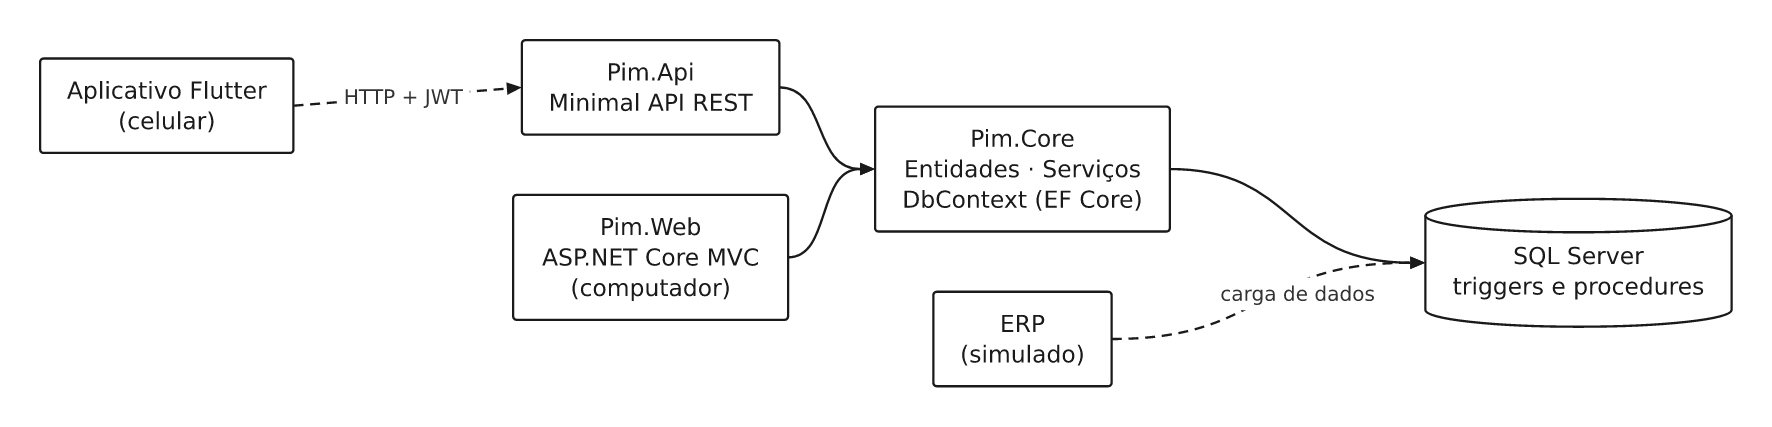
\includegraphics{figuras/arquitetura.png}
\fonte{Elaborado pelo autor (2026)}
\end{figure}

Dentro do núcleo, o domínio tem quatro contextos com vocabulário e regras próprios \cite{evans2016}: \textbf{Entrada} (recebimentos, caixas e etiquetas), \textbf{Frota} (veículos e motoristas), \textbf{Expedição} (carregamentos, portaria, entregas e retornos) e \textbf{ERP} (cópia de clientes, notas e pedidos). Hoje eles convivem em um único projeto e \texttt{DbContext}, o que basta ao tamanho atual (ver Seção~\ref{sec:evolucao}).

\section{Orientação a objetos e recursos modernos do C\#}

As entidades encapsulam dados e comportamentos do domínio \cite{wazlawick2014}. A classe \texttt{Motorista} expõe o método \texttt{CnhValidaEm(data)}, de modo que a regra RN18 é perguntada ao próprio objeto, e \texttt{PedidoVenda.TotalCaixas} é uma propriedade calculada a partir dos itens. Situações e status são enumerações, o que impede valores inválidos. A herança aparece na \texttt{RegraNegocioException}, especialização de \texttt{Exception} que sinaliza violação de regra, e o polimorfismo na sobrescrita de \texttt{OnModelCreating} do \texttt{DbContext}. Os serviços consultam esses objetos antes de qualquer gravação e, a cada violação, lançam a exceção com o código da regra, como ``RN17: veículo em manutenção''.

Dos recursos modernos da linguagem \cite{deitel2017}, os \textit{records} são usados em todos os dados que trafegam entre camadas, como \texttt{LinhaConferencia}, \texttt{EntregaPedido} e os DTOs da API. Eles são imutáveis e comparados pelo valor. O mapeamento de entidade para DTO é feito à mão, com \texttt{Select(item => new LinhaConferencia(...))}: fica explícito no código o que sai de cada consulta, sem bibliotecas que dependam de reflexão. Os tipos de referência anuláveis estão ativados nos três projetos (\texttt{<Nullable>enable</Nullable>}): \texttt{string? Motivo} declara que o motivo é opcional, e o compilador avisa quando um valor possivelmente nulo é usado sem verificação. Já os atributos de validação (Capítulo~\ref{cap:web}) são lidos por reflexão pelo próprio ASP.NET Core.

\section{Coleções, LINQ e acesso a dados}

O LINQ é usado de duas formas. Sobre coleções já carregadas em memória (\texttt{IEnumerable<T>}), como em \texttt{TotalCaixas}, os operadores executam em C\#. Sobre o \texttt{DbContext} (\texttt{IQueryable<T>}), a consulta é apenas descrita e só executa ao ser materializada, por exemplo com \texttt{ToListAsync}; até lá, ela pode ser composta. A lista de pedidos usa essa execução adiada para acrescentar filtros apenas quando informados, gerando um único comando SQL só com as condições necessárias.

\begin{codeblock}[Consulta composta com execução adiada (Pim.Web/Controllers/PedidosController.cs)]{[Sharp]C}
var consulta = _db.PedidosVenda.Include(p => p.Cliente)
                              .Include(p => p.Itens).AsQueryable();
if (status != null)
    consulta = consulta.Where(p => p.Status == status); // nao executa
if (!string.IsNullOrWhiteSpace(busca))
    consulta = consulta.Where(p => p.Cliente!.Nome.Contains(busca));
var pedidos = await consulta.OrderByDescending(p => p.DataEmissao)
                            .ToListAsync();   // um SELECT aqui
\end{codeblock}

Por padrão, o EF Core rastreia as entidades lidas para detectar alterações, o que é necessário nos serviços que gravam. Nas telas apenas de leitura, como as listas do Web, o \texttt{AsNoTracking} reduziria memória e processamento, e as projeções feitas diretamente na consulta (\texttt{Select} antes do \texttt{ToListAsync}) trariam do banco só as colunas usadas, em vez de entidades completas com \texttt{Include}. Elas e as consultas compiladas ficaram como melhorias, pois as medições (Seção~\ref{sec:desempenho}) não indicaram necessidade.

\section{Injeção de dependência e padrões de projeto}

A Inversão de Controle faz com que nenhuma classe crie suas dependências: os \textit{controllers} as recebem no construtor, e as rotas da API, como parâmetros do método. O contêiner nativo do ASP.NET Core resolve cada uma conforme o tempo de vida registrado. O \texttt{PimDbContext} e todos os serviços de regra são \textit{scoped}: há uma instância por requisição, e os serviços da mesma requisição compartilham o mesmo \texttt{DbContext} e, portanto, a mesma transação. A chave de assinatura do JWT é \textit{singleton}, pois é imutável e igual para toda a aplicação; não há serviços \textit{transient}. Um \textit{singleton} nunca depende de um \textit{scoped}, pois manteria preso um \texttt{DbContext} de uma requisição já encerrada.

Os padrões aplicados são \textbf{MVC}, \textbf{Camada de Serviço}, \textbf{Unidade de Trabalho} e \textbf{Repositório} (providos pelo \texttt{DbContext}) \cite{fowler2006}, \textbf{Injeção de Dependência}, \textbf{DTO} e \textbf{tratamento centralizado de erros}.

\section{Desempenho e diagnóstico}
\label{sec:desempenho}

O princípio adotado foi medir antes de otimizar. O caminho mais executado (\textit{hot path}) é a bipagem, e ele é limitado por entrada e saída: quase todo o tempo é gasto esperando o banco. Por isso, toda a cadeia é assíncrona, da rota ao EF Core, liberando a \textit{thread} enquanto a consulta não volta. Técnicas de redução de alocação, como \texttt{Span<T>} e \textit{pooling}, atuam no processamento em memória e não alterariam o que o usuário percebe nesse cenário.

Para verificar o requisito de resposta abaixo de um segundo, um \textit{script} de medição (testes/\allowbreak medir\_latencia.py) executa 20 bipagens de aquecimento e depois 500 bipagens em sequência, como um conferente, em base zerada. A média esconde as respostas lentas, por isso foram usados percentis: o p95 é o tempo abaixo do qual ficam 95\% das respostas. A Tabela~\ref{tab:latencia} mostra o resultado em ambiente local (notebook, com SQL Server em contêiner).

\begin{table}[htbp]
\centering
\caption{Latência medida da bipagem de entrada (500 requisições)}
\label{tab:latencia}
\footnotesize
\begin{tabular}{|c|c|c|c|c|c|}
\hline
\textbf{Média} & \textbf{p50} & \textbf{p95} & \textbf{p99} & \textbf{Máximo} & \textbf{Meta} \\ \hline
12,7 ms & 12,2 ms & 17,3 ms & 22,6 ms & 46,3 ms & < 1.000 ms \\ \hline
\end{tabular}
\fonte{Elaborado pelo autor (2026)}
\end{table}

Com o p99 cerca de 40 vezes abaixo da meta, micro-otimizações não se justificam. Como a medição é sequencial, o próximo passo é um teste de carga com vários conferentes, acompanhado pelo \texttt{dotnet-counters} (requisições por segundo, \textit{thread pool} e coleta de lixo) e, se o p99 piorar, pelo \texttt{dotnet-trace}. Esse teste deve expor uma limitação conhecida de concorrência: o código da etiqueta é gerado como ``maior código existente + 1''. Duas bipagens no mesmo instante podem calcular o mesmo número; o índice único impede a duplicação (RN01), mas a segunda requisição falha. A correção prevista é gerar o número por uma \texttt{SEQUENCE} do SQL Server, atômica por definição.

\section{Tempo real, cache e versionamento}

Hoje, a tela de um carregamento mostra o progresso ao ser carregada. Com o SignalR, o serviço notificaria, pelo \texttt{IHubContext}, o grupo \texttt{carregamento-7}, e cada bipagem apareceria na hora para quem acompanha aquele carregamento; o cliente, com reconexão automática, recarregaria o estado ao reconectar. Com várias instâncias do Web, seria preciso um \textit{backplane}, como o Azure SignalR Service.

Os dados operacionais mudam a cada bipagem, e um cache de resposta no servidor mostraria situações vencidas. Já dados de referência, como a lista de veículos, poderiam usar \textit{ETags}: com \texttt{If-None-Match}, o cliente recebe \texttt{304 Not Modified}, sem corpo, quando nada mudou; com \texttt{If-Match}, quem tentar gravar sobre uma versão desatualizada recebe \texttt{412}.

Como o aplicativo nos celulares é atualizado mais devagar que o servidor, a API só evolui com mudanças compatíveis, como novos campos opcionais; uma mudança incompatível iria para um novo grupo de rotas (\texttt{/v2}), mantido em paralelo até a atualização de todos os aparelhos.

\section{Qualidade contínua}

A pirâmide de testes recomenda muitos testes de unidade, menos de integração e poucos de ponta a ponta. Na solução, a camada mais forte é a de integração: 84 verificações por HTTP contra o Web e a API reais (Capítulo~\ref{cap:resultados}). O \textit{script} de execução dos testes (rodar.sh) apaga e recria a base \texttt{PimDbTeste} a cada execução, aplicando o conceito de banco de dados efêmero: todo teste parte do mesmo estado conhecido, sem tocar na base de desenvolvimento. O aplicativo tem testes de unidade e um de ponta a ponta. Faltam testes de unidade dos serviços em C\# e testes dentro do processo. A evolução prevista é um projeto xUnit com o \texttt{WebApplicationFactory}, que sobe a API em memória, e o Testcontainers, que cria um SQL Server descartável. Na análise estática, os avisos de nulidade já são emitidos; o passo seguinte é um arquivo de regras de estilo (.editorconfig) com as regras dos analisadores Roslyn e avisos tratados como erro na integração contínua, para que a revisão automatizada barre o código antes da revisão humana.

\section{Estratégias de manutenção e evolução}
\label{sec:evolucao}

A manutenção é apoiada pelas \textit{migrations}, pelos testes automatizados e pela documentação OpenAPI. Para a evolução, o caminho previsto é transformar a solução em um \textbf{monólito modular}, com cada contexto da Seção~\ref{sec:camadas} em um projeto próprio e três regras: tudo é \texttt{internal}, exceto um contrato público (por exemplo, \texttt{IFrotaApi}), de modo que o compilador impede que um módulo acesse as classes de outro; cada módulo tem os seus próprios dados, sem chave estrangeira entre módulos; e um módulo guarda a cópia dos dados de que precisa no momento do uso, como a placa do veículo na expedição. Os módulos seguiriam em um único processo, ligados por injeção de dependência.
